\documentclass[conference]{IEEEtran}
\IEEEoverridecommandlockouts
% The preceding line is only needed to identify funding in the first footnote. If that is unneeded, please comment it out.
\usepackage{cite}
\usepackage{amsmath,amssymb,amsfonts}
\usepackage{algorithmic}
\usepackage{graphicx}
\usepackage{textcomp}
\usepackage{xcolor}
\def\BibTeX{{\rm B\kern-.05em{\sc i\kern-.025em b}\kern-.08em
    T\kern-.1667em\lower.7ex\hbox{E}\kern-.125emX}}
\begin{document}

\title{CECS: A Concurrent Entity Component System}

\author{\IEEEauthorblockN{Voor}
\IEEEauthorblockA{\textit{College of Eng. and Computer Science}\\
\textit{University of Central Florida}\\
Orlando, Florida \\
jamesvoor@knights.ucf.edu}
\and
\IEEEauthorblockN{Bramham}
\IEEEauthorblockA{\textit{College of Eng. and Computer Science} \\
\textit{University of Central Florida}\\
Orlando, Florida \\
connor.bramham@knights.ucf.edu}
\and
\IEEEauthorblockN{Vargas}
\IEEEauthorblockA{\textit{College of Eng. and Computer Science} \\
\textit{University of Central Florida}\\
Orlando, Florida \\
angel0615@knights.ucf.edu}
}

\maketitle

\begin{abstract}
The CECS is a project which implements concurrent programming concepts
to meet the performance needs of modern simulated world applications. We discuss 
the correct program behavior of an Entity-Component-System, and the challenges
associated with parallelizing this program behavior. We discuss the successes 
of previous entity-component-system projects, and opportunities we identified which could improve performance. We discuss how our ECS system compares to established work in the field. 
\end{abstract}

\begin{IEEEkeywords}
concurrent, entity-component-system, parallelized, work-stealing
\end{IEEEkeywords}

\section{Introduction}
what is an ecs here

\section{our ECS model}
TO DO
...

\subsection{example subheading}

\begin{figure}[htbp]
\centerline{\includegraphics[scale=.4]{ECS_Diagrams.png}}
\caption{ECS diagram}
\label{ECS diagram label}
\end{figure}
\begin{figure}[htbp]
\centerline{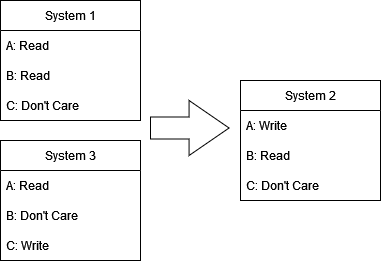
\includegraphics[scale=.4]{parallel_systems.png}}
\caption{Example of a parallel systems caption.}
\label{label for parallel systems}
\end{figure}
\begin{figure}[htbp]
\centerline{\includegraphics[scale=.4]{serial_systems.png}}
\caption{Example of a serial systems caption.}
\label{label for serial systems}
\end{figure}
\begin{figure}[htbp]
\centerline{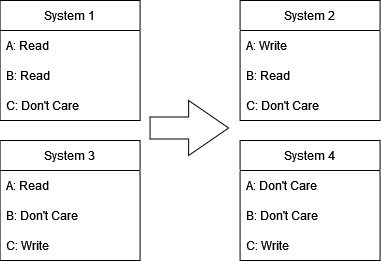
\includegraphics[scale=.4]{work_stealing.png}}
\caption{Example of a work stealing caption.}
\label{label for work stealing}
\end{figure}

\section{further model discussion}
drink coffee, ill take a cuppachino thanks

\subsection{example part a}
TO DO
\subsection{correct program behavior}
\begin{itemize}
\item item1
\item behavior2
\item behavior3
\item behavior4
\end{itemize}

\subsection{methods for parallelizing}
great explanation goes here
\begin{equation}
a+b=\gamma\label{eq}
\end{equation}

continue excellent explanation 

\section{Review of related work}
talk about em here...

\subsection{Figures and Tables}
\paragraph{Positioning Figures and Tables} Place figures and tables at the top and 
bottom of columns. Avoid placing them in the middle of columns. Large 
figures and tables may span across both columns. Figure captions should be 
below the figures; table heads should appear above the tables. Insert 
figures and tables after they are cited in the text. Use the abbreviation 
``Fig.~\ref{ECS diagram label}'', even at the beginning of a sentence.

\begin{table}[htbp]
\caption{Table Type Styles}
\begin{center}
\begin{tabular}{|c|c|c|c|}
\hline
\textbf{Table}&\multicolumn{3}{|c|}{\textbf{Table Column Head}} \\
\cline{2-4} 
\textbf{Head} & \textbf{\textit{Table column subhead}}& \textbf{\textit{Subhead}}& \textbf{\textit{Subhead}} \\
\hline
copy& More table copy$^{\mathrm{a}}$& &  \\
\hline
\multicolumn{4}{l}{$^{\mathrm{a}}$Sample of a Table footnote.}
\end{tabular}
\label{tab1}
\end{center}
\end{table}

Figure Labels: Use 8 point Times New Roman for Figure labels. Use words 
rather than symbols or abbreviations when writing Figure axis labels to 
avoid confusing the reader. As an example, write the quantity 
``Magnetization'', or ``Magnetization, M'', not just ``M''. If including 
units in the label, present them within parentheses. Do not label axes only 
with units. In the example, write ``Magnetization (A/m)'' or ``Magnetization 
\{A[m(1)]\}'', not just ``A/m''. Do not label axes with a ratio of 
quantities and units. For example, write ``Temperature (K)'', not 
``Temperature/K''.

\section*{Acknowledgment}

The preferred spelling of the word ``acknowledgment'' in America is without 
an ``e'' after the ``g''. Avoid the stilted expression ``one of us (R. B. 
G.) thanks $\ldots$''. Instead, try ``R. B. G. thanks$\ldots$''. Put sponsor 
acknowledgments in the unnumbered footnote on the first page.

\section*{References}

Please number citations consecutively within brackets \cite{b1}. The 
sentence punctuation follows the bracket \cite{b2}. Refer simply to the reference 
number, as in \cite{b3}---do not use ``Ref. \cite{b3}'' or ``reference \cite{b3}'' except at 
the beginning of a sentence: ``Reference \cite{b3} was the first $\ldots$''

Number footnotes separately in superscripts. Place the actual footnote at 
the bottom of the column in which it was cited. Do not put footnotes in the 
abstract or reference list. Use letters for table footnotes.

Unless there are six authors or more give all authors' names; do not use 
``et al.''. Papers that have not been published, even if they have been 
submitted for publication, should be cited as ``unpublished'' \cite{b4}. Papers 
that have been accepted for publication should be cited as ``in press'' \cite{b5}. 
Capitalize only the first word in a paper title, except for proper nouns and 
element symbols.

For papers published in translation journals, please give the English 
citation first, followed by the original foreign-language citation \cite{b6}.

\begin{thebibliography}{00}
\bibitem{b1} G. Eason, B. Noble, and I. N. Sneddon, ``On certain integrals of Lipschitz-Hankel type involving products of Bessel functions,'' Phil. Trans. Roy. Soc. London, vol. A247, pp. 529--551, April 1955.
\bibitem{b2} J. Clerk Maxwell, A Treatise on Electricity and Magnetism, 3rd ed., vol. 2. Oxford: Clarendon, 1892, pp.68--73.
\bibitem{b3} I. S. Jacobs and C. P. Bean, ``Fine particles, thin films and exchange anisotropy,'' in Magnetism, vol. III, G. T. Rado and H. Suhl, Eds. New York: Academic, 1963, pp. 271--350.
\bibitem{b4} K. Elissa, ``Title of paper if known,'' unpublished.
\bibitem{b5} R. Nicole, ``Title of paper with only first word capitalized,'' J. Name Stand. Abbrev., in press.
\bibitem{b6} Y. Yorozu, M. Hirano, K. Oka, and Y. Tagawa, ``Electron spectroscopy studies on magneto-optical media and plastic substrate interface,'' IEEE Transl. J. Magn. Japan, vol. 2, pp. 740--741, August 1987 [Digests 9th Annual Conf. Magnetics Japan, p. 301, 1982].
\bibitem{b7} M. Young, The Technical Writer's Handbook. Mill Valley, CA: University Science, 1989.
\end{thebibliography}
\vspace{12pt}
\color{red}
IEEE conference templates contain guidance text for composing and formatting conference papers. Please ensure that all template text is removed from your conference paper prior to submission to the conference. Failure to remove the template text from your paper may result in your paper not being published.

\end{document}
